\section{Arquitetura do Sistema}
\subsection{Extensão do \textit{becnhmark}}
\subsection{A Arquitetura}

O objetivo desta arquitetura é fornecer uma estrutura de mecanismos automáticos de gerenciamento de desempenho de um conjunto de recursos físicos.

, contratados junto
a um provedor de nuvem, por um consumidor de IaaS, que utiliza a infraestrutura contratada para
entregar algum tipo de serviço (i. e PaaS ou SaaS) a seus clientes ou usuários finais.
Nesse formato de negócio, o provedor de nuvem detém a propriedade de recursos computacionais
altamente escaláveis dispostos em data centers geograficamente dispersos acessíveis pela
Internet. Comumente, o provedor aluga servidores virtualizados nessa infraestrutura física para
seus consumidores em um modelo de pagamento por uso. Nesse modelo os consumidores são
onerados apenas quando os recursos, frequentemente representados por máquinas virtuais, estão
sendo utilizados. Por sua vez, o consumidor dos serviços de nuvem aplica as máquinas virtuais
contratadas para oferecer algum tipo de serviço Web para usuários finais, eventualmente, cobrando
esses usuários pelo acesso ao serviço dando em troca a garantia da qualidade do serviço prestado.
Há diferenças substanciais entre os valores cobrados pelo provedor para máquinas virtuais ligadas
e em execução, que utilizam processamento, memória e rede; e desligadas, quando utilizam
apenas espaço em disco para armazenamento. Usualmente, os custos relativos ao armazenamento
são mais baixos que para os demais recursos que podem ser adquiridos junto ao provedor, sendo
dispendioso manter máquinas virtuais ligadas quando as mesmas não são necessárias no atendimento
da demanda gerada pelas requisições enviadas pelos usuários do serviço.
Para ter um rendimento adequado, o consumidor deve manter, ou mesmo otimizar, um ponto
de equilíbrio entre a quantidade de recursos consumidos pelos quais está pagando e a demanda
gerada por seus clientes pela qual está cobrando, além de que o descumprimento dos contratos
junto aos usuários finais pode ocasionar a redução dos ganhos. Para isso, é necessário gerenciar
o desempenho dos recursos disponíveis para que haja um mínimo perdas por descumprimentos de
contratos. A figura 4.1 ilustra em alto nível os principais componentes da arquitetura proposta.
A arquitetura considera um ambiente usual de computação em nuvem como mostrado na figura
1.1, com duas formas principais de interação entre as partes envolvidas: negócio e comunicação.
A interação que compõe a linha do negócio refere-se ao que é estabelecido por contrato entre os
envolvidos e motiva a orientação a mercado dada para arquitetura, já que usualmente os serviços
em nuvem são pagos. Como a arquitetura proposta é orientada ao mercado, alguns módulos são
comuns aos propostos por Buyya et al. (2008) para um controle de admissão em data centers.
A linha da comunicação envolve o envio de requisições pelos usuários e de respostas pelas máquinas
virtuais no data center. O consumidor não participa dessa interação que é feita diretamente
entre os clientes que acessam os serviços hospedados na infraestrutura contratada.

\begin{figure}[!htb]
	\caption{Arquitetura do experimento}
	\label{fig:arquitetura-experimento}
	\centering
	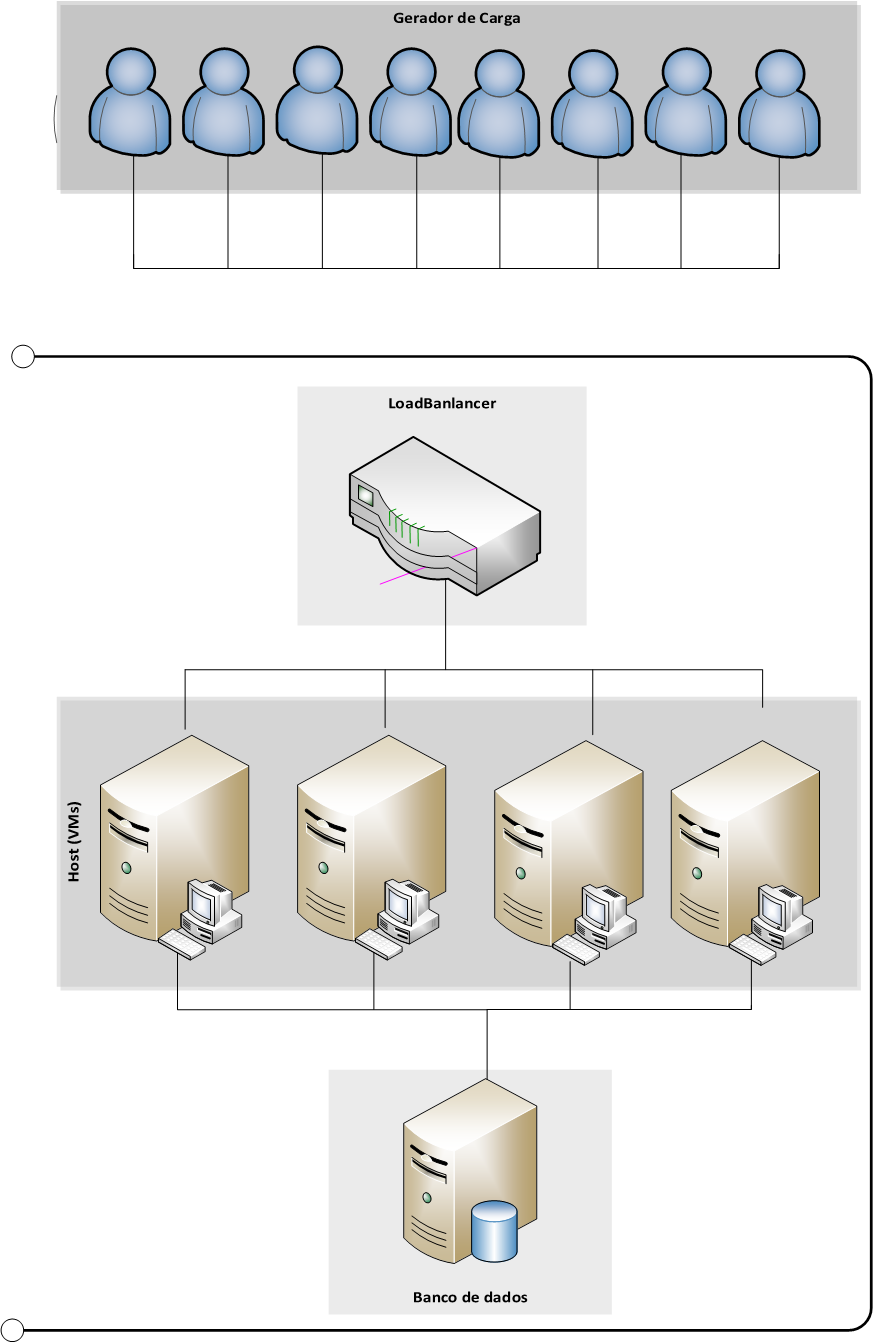
\includegraphics[scale=0.6]{arquitetura-experimento.png}
	\fautor
\end{figure}

Comumente a avaliação de desempenho de sistemas computacionais é realizada em regime estacionário, isto é, sob carga de trabalho constante.  O sistema inicialmente sem carga, é excitado com a entrada de interesse, e aguarda-se até que a saída estabilize-se no valor desejado, podendo ser um valor constante ou um valor dentro de um intervalo. A condição aceitável é alcançada passado o \textit{warm up} (aquecimento), período em que o sistema encontra-se em estado de inicialização. A determinação da capacidade obtém-se estimulando o sistema com carga gradativamente mais elevadas até atingir seu limite inferior de desempenho aceitável, correspondente à carga estática máxima suportada. Análise do comportamento no período de aquecimento contém informações importantes relacionadas com a capacidade do sistema operando em condições reais onde a carga não é constante.
Em regime transiente, a quantidade de recursos necessários para garantir o desempenho especificado pode divergir substancialmente daquela definida em regime estacionário. Durante um período transiente, as consequências de uma perturbação na carga a quantidade de recursos necessários seria temporariamente superior àquela prevista para o regime de carga não variável. Isso resulta, por exemplo, em descumprimento dos níveis de serviço ou paradas no funcionamento dos sistemas.
%Dentro de um ambiente de testes local uma das principais limitações na simulação de sistemas e-commerce é o acesso ao banco de dados. Percebe-se que o banco de dados é o principal fator limitante para a analise transiente  para níveis altos de carga os dados coletados são pouco uteis, porque aparecem claros sinais de problemas de entrada e saída. 

\section{Experimentos}
\subsection{Ambiente de Experimentação}
O ambiente utilizado para execução dos experimentos é apresentado na Tabela \ref{tab:configuracao_maquinas}.
Foram utilizadas oito unidades para a geração de carga \textit{workload} que atuam como clientes dos
serviços, uma unidade de balanceamento de carga e 4 servidores atuando como provedor de serviços e uma
unidade executando o banco de dados a ser consultado pelo provedor de serviços.
%Considerando que há uma quantidade máxima de N clientes no sistema, cada equipamento cliente executa simultaneamente N/4 aplicações clientes ou processos

\begin{table}[htb]
	\centering
	\caption{Especificação do ambiente de execução dos experimentos}
	\label{tab:configuracao_maquinas}
	\begin{tabularx}{\textwidth}{r|c|X} \hline\hline
		\textbf{Componente}    & \textbf{Quantidade} & \textbf{Configuração} \\ \hline
		\textit{Workload}      & 8 Unidades          & Intel Core 2 Quad Q6600 2.4GHz, 4GB de RAM \\
		\textit{Load Balancer} & 1 Unidade           & Intel Core 2 Quad Q6600 2.4GHz, 4GB de RAM \\
		\textit{Hosts}         & 4 Unidade           & Intel Core 2 Quad Q6600 2.4GHz, 4GB de RAM \\
		\textit{Data base}     & 1 Unidade           & Intel Core 2 Quad Q6600 2.4GHz, 4GB de RAM \\
		\hline
	\end{tabularx}
	\fdadospesquisa
\end{table}


\subsection{Planejamento de Experimentos}
Os experimentos conduzidos neste trabalho consideraram três diferentes fatores de dois níveis cada, conforme aprestando na Tabela \ref{tab:fatores_niveis}. 

\begin{table}[htb]
	\centering
	\caption{Fatores e níveis dos experimentos}
	\label{tab:fatores_niveis}
	\begin{tabularx}{\textwidth}{c|c|c|c} \hline\hline
        Fatores  & \textit{Workload} & Banco de dados \\ \hline
		Nível 1  &         			 & Postgres \\
		Nível 2  &            		 & DB2 \\
		\hline
	\end{tabularx}
	\fdadospesquisa
\end{table}


O primeiro fator refere-se à quantidade de clientes simultâneos requisitando serviços ao
Serviço Web, considerando-se duas quantidades: 100 e 170 clientes. O segundo fator
está associado ao processo de chegada das requisições, ou seja, a política de geração de
think times a ser adotada, para situações sem ou com rajadas. O terceiro fator considera
a demanda de serviço imposta ao Serviço Web, desconsiderando o tempo de consulta ao
banco de dados. Esse fator representa a possibilidade de serem considerados diferentes
tipos de serviço, com demanda computacional distintas. Para esse fator são atribuídos
dois níveis: uma demanda de serviço básica, associada ao tempo médio de serviço para
que as requisições sejam concluídas pelo Serviço Web e uma demanda de serviço até
67% mais alta do que o tempo médio de serviço básico. Por último, o quarto fator
refere-se ao tamanho da base de dados a ser consultada pelo Serviço Web, base BDLeve
ou BDPesada. Os níveis dos fatores considerados apresentam um aumento equivalente em
torno de 70% de um nível para o outro. Esse aumento foi escolhido com o objetivo de
manter uma diferença equilibrada entre todos os valores dos níveis de cada fator.
O planejamento de experimentos utilizado na avaliação de desempenho
apresentada neste artigo segue a abordagem do planejamento fatorial completo. Esta
abordagem foi escolhida por possibilitar que todas as combinações possíveis de
configurações e cargas de trabalho sejam examinadas. Para todos os experimentos
foram realizadas 5 execuções, cada uma com duração aproximada de 40 minutos,
utilizadas para determinar a média, o desvio padrão e o intervalo de confiança de 95%
de acordo com a tabela T-student. O número de execuções e duração foi definido
considerando-se a necessidade de obter diferença significativa dentre os intervalos de
confiança dos experimentos que implica em comparação dos resultados. Os
experimentos foram conduzidos com o objetivo de avaliar aspectos relacionados ao
desempenho do serviço, compreendendo as seguintes variáveis de resposta:
Tempo médio de resposta: intervalo de tempo entre o envio da requisição pelo
cliente e chegada da resposta completa processada pelo Serviço Web;
Tempo médio de execução WS: tempo médio de execução das requisições
processadas pelo Serviço Web, incluindo tempo médio consumido para estabelecer
as conexões com o banco de dados; 

\subsection{Avaliação de desempenho em regime transiente}





Para iniciar o desenvolvimento de extensão do Bench4Q, iniciamos por trabalhar com uma versão completa da implementação do \textit{benchmark} Bench4Q \textbf{(adicionar link de download da ferramenta)}
----------------------------

Agora que a metodologia de extensão esta definida, apresenta-se um caso de estudo prático que demonstra como ela pode ser usada e aplicada para analisar o desempenho transiente de um sistema. Caso de estudo é uma metodologia ideal quando um holístico, investigação aprofundada é necessária %(Feagin, Orum, & Sjoberg, 1991). 

\section{O protocolo de caso de estudo}
Considere uma livraria que desejar realizar uma promoção no dia de seu aniversario, essa promoção é ousada e espera-se ter um grande volume de vendas decorre a comemoração, isso irá apoiar as suas operações de venda e expandir seu mercado. Logo, a maior preocupação por parte da empresa é que seu \textit{e-commerce} esteja disponível para os compradores/clientes, assim a empresa decidiu contratar os serviços de uma provedora de \textit{Cloud Computing} para hospedar o seu \textit{e-commerce} no dia o evento. O ambiente destinado para este evento está em processo de validação de carga, por parte da operadora, para garantir que os clientes antigos e novos da livraria possam usufruir e aproveitarem a promoção, e para a provedora não correr o risco de perderem o contrato o diretor de TI da provedora solicitou a sua equipe de engenheiros realizarem experimentos para garantir o desempenho esperado pelo cliente contrante.
Supondo que, em condições normais de funcionamento, o \textit{e-commerce} da livraria tem 10 clientes simultâneos e durante o dia do evento da mega promoção de aniversario, espera-se em média 20 clientes simultâneos,  além disso, a carga de trabalho está prevista para crescer em até 300\% ao longo do dia. A empresa contrante, a livraria, acredita que o tempo médio de resposta para todas as operações é de 7 segundos, e deseja que 90\% dos seus clientes estejam dentro dessas condições pré estabelecidas por ela, ou seja, a livraria da um margem de 10\% dos cliente fiquem fora do desempenho definido. Note-se que todos estes números e valores foram escolhidos de forma arbitrária, de modo a tornar o nosso cenário motivador mais específico.
Ao ler os requisitos de desempenho, a equipe de engenheiros, vez a necessidade de uma analise transiente, que por sua vez, buscam um \textit{becnhmark} para realizar os experimentos, então identificam um \textit{becnhmark} que se adéqua-se ao caso, entretanto o \textit{becnhmark} em questão não realiza analise transiente, contudo a equipe decide em aplicar a metodologia proposta neste trabalho.

Ainda assim, a equipe de engenheiro da operadora de \textit{Cloud Computing} precisa garantir e encontrar respostas para as seguintes perguntas, após a aplicação da metodologia:

\begin{itemize}
	\item Com a aplicação da metodologia, o \textit{becnhmark} irá estimular o sistema a apresentar a sua dinâmica, permitindo a analise em regime transiente do mesmo? 
	\item Que as métricas utilizadas pelo contratante são sendo analisadas
\end{itemize}

%Para um determinado número de servidores WebLogic, qual o nível de desempenho que o sistema fornece?

%Quantos servidores WebLogic seriam necessários para garantir o desempenho adequado sob a carga de trabalho esperada?

%Será que a capacidade do balanceador de carga e único servidor de banco de dados único suficiente para lidar com a carga de entrada?

%Será que a escala do sistema ou existem outros gargalos do sistema potencial?

%Vamos supor que o primeiro protótipo desta aplicação é SPECjAppServer2004 e que a empresa está testando a aplicação no ambiente de implantação mostrado na Figura 6.6. Este ambiente usa um cluster de servidores WebLogic (WLS) como um recipiente J2EE e um servidor de banco de dados Oracle (DBS) para persistência. Assumimos que todos os servidores no cluster WebLogic são idênticos e que, inicialmente, apenas dois servidores estão disponíveis.

%Com base nessas premissas, as seguintes metas concretas são estabelecidos:

%Prever o desempenho do sistema em condições normais de funcionamento com 4 e 6 servidores WebLogic, respectivamente. Qual seria o rendimento da transação média e tempo de resposta (para procurar, comprar e gerenciar)? Quantas trabalho ordens seria concluída por segundo no domínio de fabricação e qual seria o tempo médio de processamento da ordem de serviço? Como utilizada (CPU / utilização de disco) seriam os servidores WebLogic, o balanceador de carga eo servidor de banco de dados?

%?? Determinar se seis servidores WebLogic seria suficiente para garantir que os tempos médios de resposta de transações de negócios não exceda metade de um segundo durante condições de pico.

%?? Prever o quanto o desempenho do sistema poderia melhorar se o balanceador de carga é atualizado com um CPU um pouco mais rápido.

%?? Estudar a escalabilidade do sistema com o aumento da carga de trabalho e servidores WebLogic adicionais são adicionados.

%?? Determinar quais servidores seriam mais utilizados sob carga pesada e investigar se eles são potenciais pontos de estrangulamento. Em particular, verificar se a capacidade do balanceador de carga e único servidor de banco de dados único seria suficiente para lidar com a carga de entrada.


As seções a seguir mostram como estas questões podem ser respondidas por meio da metodologia de extensão proposto, além de uma apresentação detalhada do \textit{benchmark} que fora modificado pela metodologia.

%\subsection{Limitações do Bench4Q}

%Embora bastante sofisticado, o Bench4Q é primariamente um \emph{benchmark} para avaliação de desempenho em regime estacionário, uma vez que funciona a com base na pre-configuração da carga de trabalho \emph{off-line}.  A partir do início da simulação, a carga de trabalho é iniciada com as características estocásticas predeterminadas e permanece inalterada até o final do ensaio.  Não existem provisões para a introdução de perturbações controladas durante o processo, não propiciando facilidades para a exposição das propriedades dinâmicas da planta e registro dos efeitos transientes decorrentes de variações bruscas na carga --- o que é um ponto importante do sistema de controle proposto por  \citet{Nobile2013}.


\section{Implementação da metodologia}

Nesta seção é apresentado em detalhes a implementação dos passos da metodologia, proposta no capitulo \ref{chapter:metodologia}, e aplicadas no \textit{benchmark} Bench4Q.

\begin{figure}[htb]
	\caption{Diagrama de classe modificadas e adicionadas no Bench4Q.}
	\label{fig:diagrama-classes}
	\centering
	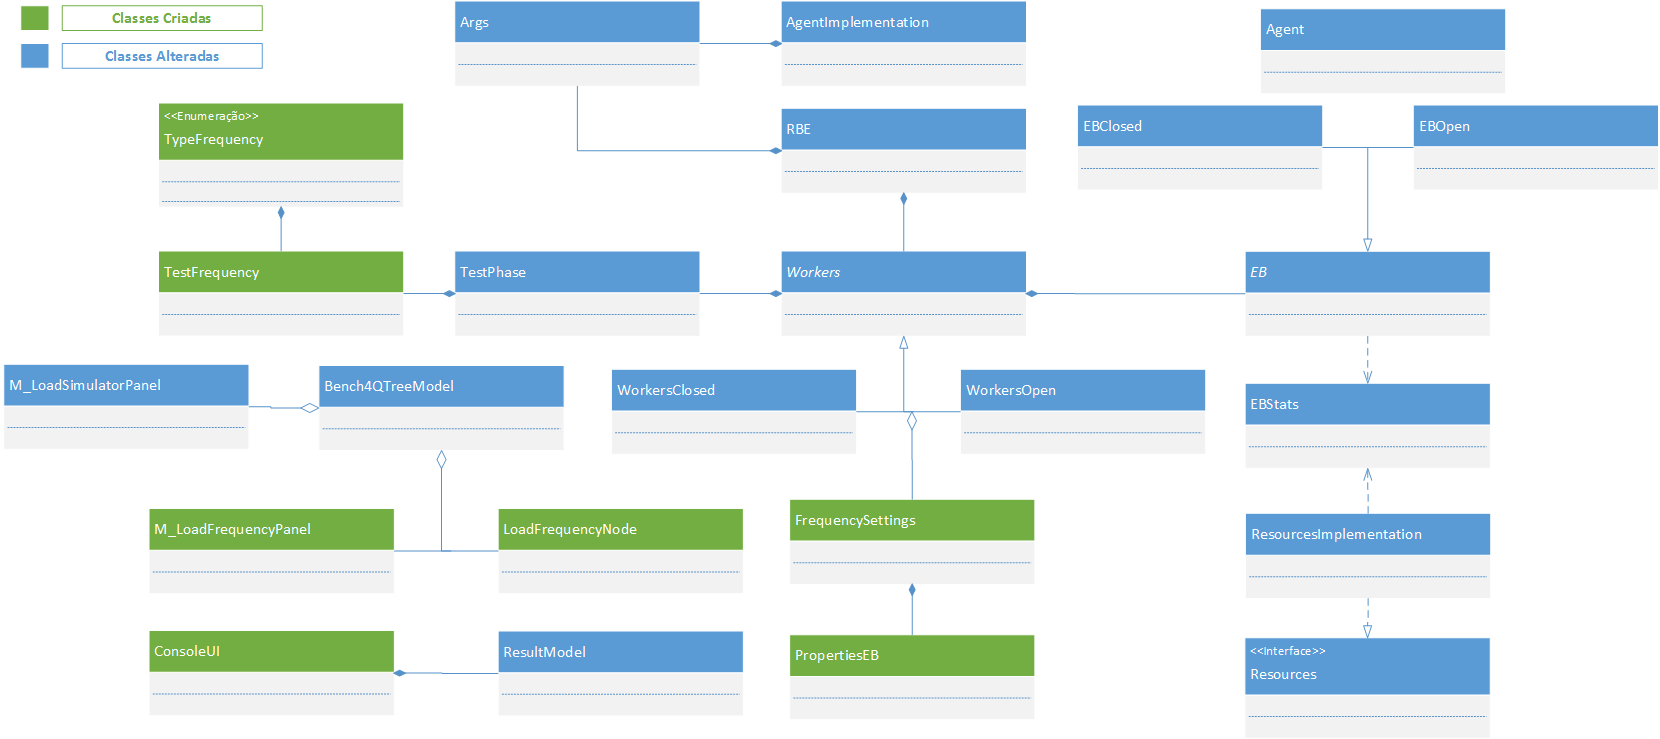
\includegraphics[scale=0.4]{diagrama-classes-beanch4Q.png}	
	%\fdireta{}
\end{figure}
	
%1º  - falar como foi implementados as modificações conforme a metodologia
Em primeiro lugar, e sem surpresa, e de acordo com a metodologia foi identificado o modulo de geração de carga do Bench4Q e este passou por alterações para gerar a carga de trabalho esperada. Conforme o diagrama de classes na figura \ref{fig:diagrama-classes}, é possível ter uma ideia do trabalho realizado no \textit{benchmark}, vale aqui salientar que o Bench4Q é uma ferramente completa e extensa, e diagramar todas as classes do mesmo ficaria difícil a sua apresentação em um único diagrama que facilita-se o entendimento, sendo assim, aqui apresentamos somente as classes já existente no Bench4Q e que passar por modificações para atender aos requisitos da metodologia e as novas classes que foram necessária para o mesmo objetivo.
%- montra diagrama de classes e diferenciando as classes existes com as que foram modificadas e adicionadas
 
	
Este conjunto de classes é que lida, manipula e gerencia a carga de trabalha gerada pelo Beanch4Q. A ferramente utiliza de um excelente console para configurar a carga de trabalho, e para mantar e respeitar o padrão do \textit{benchmark} foi implementado uma interface de configuração conforme ilustrado na figura \ref{fig:interface-criada-beanch4q}. Seguindo os padrões do Bench4Q, foi criado uma interface por onde controlar o comportamento da carga antes da execução, a carga é programada atras vezes de parâmetros informados previamente a execução do experimento. Exemplo, ao escolher a opção degrau, é necessário informar quantos EBs geram o degrau, em que instante de tempo, e qual o tempo de duração e por fim qual a sua polaridade (com base em um pulso elétrico a positiva sairia de zero e chega a um, a negativa, sairia de um e chegaria a zero).
%- mostrar a interface grafica de como ficou o Bench4Q

\begin{figure}[htb]
	\caption{Console de programação de carga de trabalho.}
	\label{fig:interface-criada-beanch4q}
	\centering
	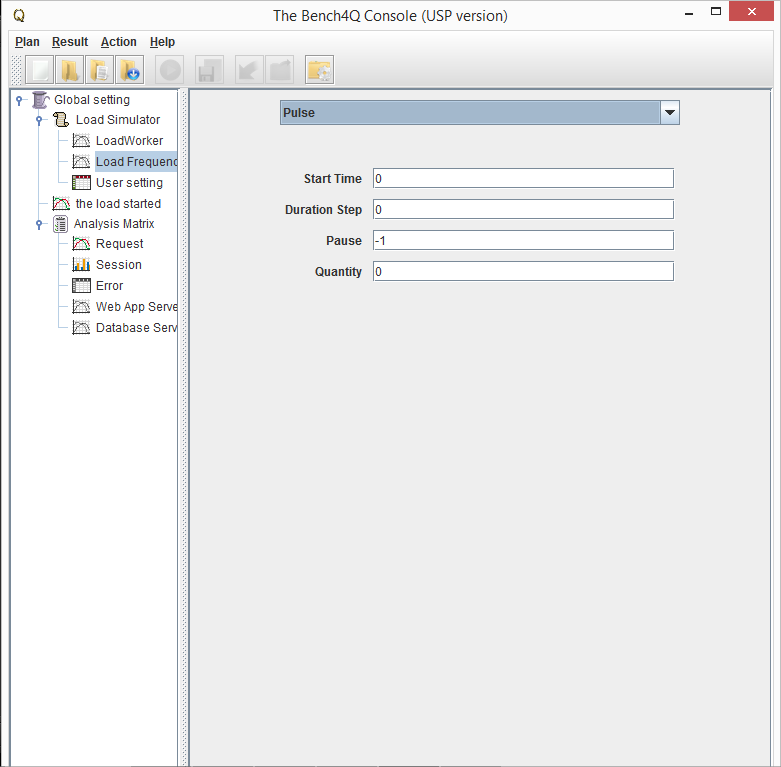
\includegraphics[scale=0.5]{console-bench4Q-usp.png}
	%\fdireta{Console de programação de carga de trabalho.}
\end{figure}
	
	
%- mostrar resultados da carga de trabalho

%2º  - falar que nao foram necessarios incluir novas metricas, pois as presentes no bench4 já são o suficiente para o estudo de caso

O Segundo passo, de acordo com a metodologia apresentada, é a definição e coleta da métrica, esta por sua vez não foi implementada, pois as métricas propostas definidas nativamente pelo Bench4Q são relevantes conforme apresentado na seção \ref{cap:caracteristicas-bench4q}.

\section{Analise dos resultados}
%3º  - mostrar a analise e o impacto do carga de trabalho no sistema  
%Podemos agora usar os resultados da análise de desempenho para atender as metas estabelecidas no ponto 6.3.1. Por meio do modelo de QPN desenvolvido, que foram capazes de prever o desempenho do sistema em condições de funcionamento normais com 4 e 6 servidores WebLogic. Descobriu-se que usando o balanceador de carga original, seis nós de servidor de aplicação não foram suficientes para garantir tempos médios de resposta de transações de negócios abaixo de meio segundo. Atualizando o balanceador de carga com um CPU ligeiramente mais rápido levou à utilização de CPU do dropping balanceador de carga por um bom 20 por cento.
%Como resultado, os tempos de resposta de transações de concessionários melhorou em 15 a 27 por cento, encontrando o "meio segundo" exigência. No entanto, o aumento da intensidade da carga de trabalho além das condições de pico revelou que o balanceador de carga foi um recurso gargalo, impedindo-nos para escalar o sistema adicionando servidores WebLogic adicionais (veja a Figura 6.14). Assim, à luz do crescimento da carga de trabalho que o esperado, a empresa deve substituir a máquina balanceador de carga com um mais rápido ou considerar o uso de um método de balanceamento de carga mais eficiente. Depois de feito isso, a análise de desempenho deve ser repetida com o novo balanceador de carga para se certificar de que não há nenhum outro gargalos do sistema. Também deve ser assegurado que o balanceador de carga é configurado com threads suficientes para que não há contenção de discussão.
%Neste capítulo, a prática metodologia de modelagem de desempenho para DCS foi apresentada.
%A metodologia aproveita o poder de modelagem e expressividade do formalismo de modelagem QPN para melhorar a representatividade do modelo e permitir a previsão de desempenho precisas. Foi apresentado um estudo de caso detalhado no qual um modelo de um DCS realista foi construído e usado para analisar o seu desempenho e escalabilidade.
%O modelo de representatividade foi validado comparando suas previsões contra medições no sistema real. Foram considerados Um número de diferentes configurações de implantação e cenários de carga de trabalho. Além disso a CPU e I / O de contenção, demonstrou-se como alguns aspectos mais complexas do comportamento do sistema, tais como a contenção de rosca e processamento assíncrono, pode ser modelado. O modelo mostrou para refletir com precisão as características do sistema de desempenho e escalabilidade em estudo. O erro de modelagem para o tempo de resposta da transação não ultrapassou 21,2% e foi muito menor para a transferência de transações e utilização de recursos. A metodologia de modelagem de desempenho proposto fornece uma ferramenta poderosa para a engenharia de DCS desempenho.

1-Projete o protocolo de estudo de caso:
	a - determinar as competências necessárias
	b - desenvolver e revisar o protocolo

2-Conduta do estudo de caso:
	a - preparar-se para a coleta de dados
	b - distribuir questionário
	c - realizar entrevistas

3 Analisar caso provas estudo:
	a - analítica estratégia

4-Desenvolver conclusões, recomendações, e as implicações com base nas provas